%\documentclass{article}
\documentclass{article}
\usepackage{times}
%\usepackage{natbib}
%\usepackage{multicol}
\RequirePackage{natbib}
\usepackage{amsmath, amssymb, fullpage, amsthm, array, algorithm2e,graphicx,asa}
%\usepackage[dvips]{graphics}

\graphicspath{{images/}}
\usepackage{color}
\newcommand{\blue}[1]{{\color{blue} #1}}
\newcommand{\red}[1]{{\color{red} #1}}

\setlength{\oddsidemargin}{0in}
\setlength{\evensidemargin}{0in}
\setlength{\textwidth}{6.5in}
\setlength{\topmargin}{-0.4in}
\setlength{\textheight}{9in}
\evensidemargin \oddsidemargin

\newtheorem{thm}{Theorem}[section]
\newtheorem{dfn}{Definition}[section]
\newtheorem{cor}{Corollary}[thm]
\newtheorem{con}{Conjecture}[thm]
%\setlength{\parindent}{0in}   % for no indent

%\topmargin -0.10in   % when making pdf
%\textheight 9.15in  % when making pdf

\setlength\parindent{0pt}

\begin{document}

% Article top matter
\title{Validation of Visual Statistical Inference, with Application to Linear Models}
\author{Mahbubul Majumder, Heike Hofmann, Dianne Cook\\
        Department of Statistics, Iowa State University}
%\date{\today}  %\today is replaced with the current date
\maketitle

\begin {abstract} 
Statistical graphics play a crucial role in exploratory data analysis, model checking and diagnosis. Until recently there were no formal visual methods in place for determining statistical significance of findings. This changed, when Buja et al. (2009) conceptually introduced two protocols for formal tests of visual findings. In this paper we take this a step further by comparing the lineup protocol (Buja et al., 2009) against classical statistical testing  of the significance of regression model parameters. A human subjects experiment is conducted using simulated data to provide controlled conditions. Results suggest that the lineup protocol provides results equivalent to the uniformly most powerful (UMP) test and for some scenarios yields better power than the UMP test.
\end {abstract}

\end{document}

%\begin{multicols}{2}
%\twocolumn

\section{Introduction} 

Any statistical analysis must include some statistical graphics. For exploratory data analysis, statistical graphics play an invaluable role in model checking and diagnostics. Even though we have established mathematical procedures to obtain various statistics, we need to support the results by also producing the relevant plots. 

The scientific foundation of graphical methods for data analysis is well established by \cite{cleveland:1984}. In recent years we have seen several major advances in statistical graphics. Modern computing systems like R and SAS tease the production of high quality statistical plots. A grammar of graphics introduced by \cite{wilkinson:1999} presents a structured way to generate specific graphics from data and define connections between disparate types of plots.  \cite{hadley:2009} has implemented a revised version of the grammar of graphics in R, in the package {\tt ggplot2}.   \blue {Graham Wills has implemented the grammar in SPSS, but I'm not sure how to cite this.}


\citet{buja:2009}, following from \cite{gelman:2004}, proposed two protocols that allow the testing of discoveries made from statistical graphics. This work represents a major advance for graphics, because it bridges the gulf between classical statistical inference procedures and exploratory data analysis.

In this paper we compare graphical inference to classical statistical inference for a set of regression type example. We also present results of a human-subject study assessing the performance of individuals on lineup plots \citep{buja:2009} for testing significance of regression parameters. 

Section \ref{sec:visual_test} describes the basic ideas of visual inference, Section \ref{sec:regression} applies these ideas to the case of inference for regression analysis. In Section \ref{sec:simulation} we outline the setup for the human-subject study and  and present results. 


\begin{table*}[hbtp]
\caption{Comparison of visual inference with existing inference technique}
\centering 
\begin{tabular}{llll} 
\hline
  & Mathematical Inference &  Visual Inference \\ %[0.5ex] % inserts table %heading 
\hline
  Hypothesis & $H_0: \beta=0$ vs $H_1: \beta \ne 0$& $H_0: \beta=0$ vs $H_1: \beta \ne 0$\\
 & \begin{minipage}[h]{1.5cm} \begin{center} \scalebox{0.2}{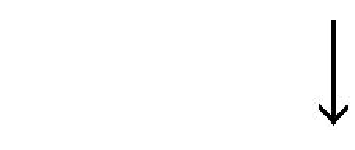
\includegraphics{down_arrow.pdf}} \end{center} \end{minipage} & \begin{minipage}[h]{1.5cm} \begin{center} \scalebox{0.2}{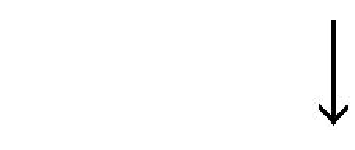
\includegraphics{down_arrow.pdf}} \end{center} \end{minipage} \\
				  
 Test statistic & $T(y)=\frac{\hat{\beta}}{se(\hat{\beta})}$ & $T(y)=$ \begin{minipage}[h]{1cm} \begin{center} \scalebox{0.15}{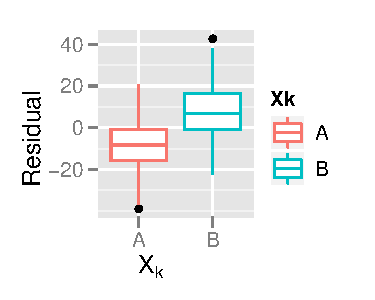
\includegraphics{stat_category.pdf}} \end{center} \end{minipage} \\
				 
 & \begin{minipage}[h]{1.5cm} \begin{center} \scalebox{0.2}{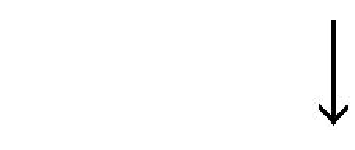
\includegraphics{down_arrow.pdf}} \end{center} \end{minipage} & \begin{minipage}[h]{1.5cm} \begin{center} \scalebox{0.2}{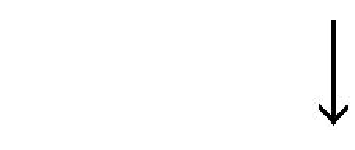
\includegraphics{down_arrow.pdf}} \end{center} \end{minipage} \\
				 
 Null Distribution & $f_{T(y)}(t); $\begin{minipage}[h]{1.5cm} \begin{center} \scalebox{0.15}{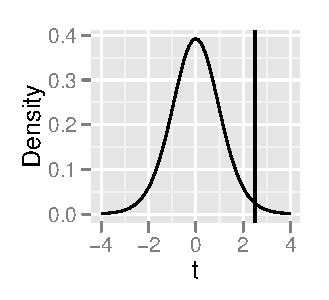
\includegraphics{stat_mathematical_test.pdf}} \end{center} \end{minipage} & $f_{T(y)}(t); $ \begin{minipage}[h]{1.5cm} \begin{center} \scalebox{0.19}{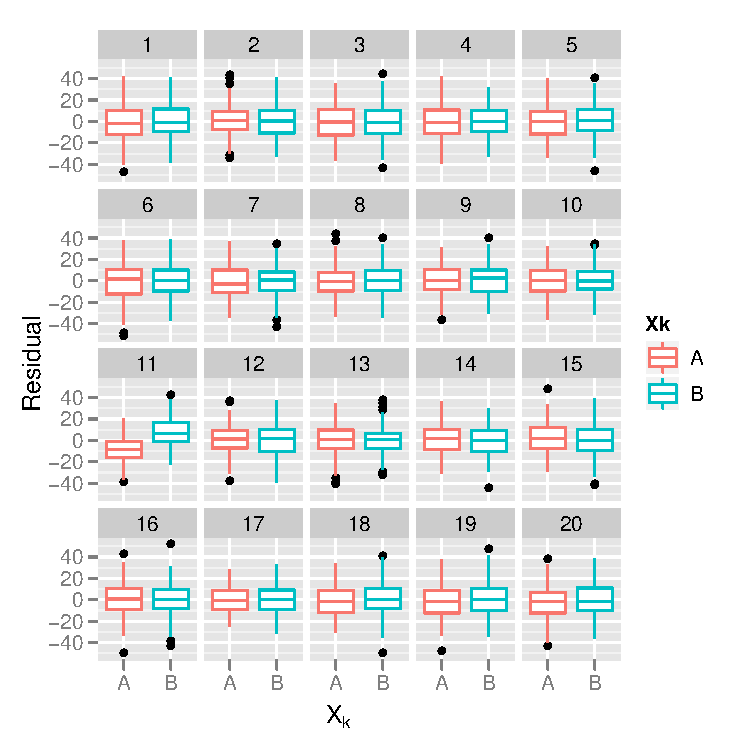
\includegraphics{test_category.pdf}} \end{center} \end{minipage} \\
 & \begin{minipage}[h]{1.5cm} \begin{center} \scalebox{0.2}{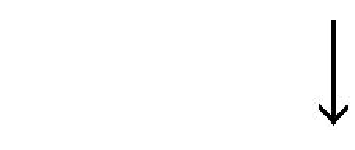
\includegraphics{down_arrow.pdf}} \end{center} \end{minipage} & \begin{minipage}[h]{1.5cm} \begin{center} \scalebox{0.2}{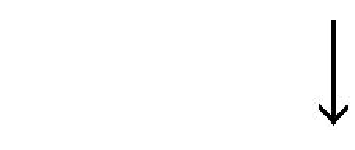
\includegraphics{down_arrow.pdf}} \end{center} \end{minipage} \\
 Reject $H_0$ if & observed $T$ is extreme & observed plot is identifiable \\
\hline 
\end{tabular}
\label{tbl:compare}
\end{table*}	

\section{Visual Statistical Inference} \label{sec:visual_test} 


This section outlines the concepts of visual inference in comparison to the procedures of classical statistical inference. Table \ref{tbl:compare} (derived from \citet{buja:2009}) gives a summarized overview of this comparison.

Let $\theta$ be a population parameter of interest, with $\theta \in \Theta$, the parameter space. 
Any null hypothesis $H_0$ then partitions the parameter space into $\Theta_0$ and $\Theta_0^c$, with $H_0: \theta \in \Theta_0$ versus $H_1: \theta \in \Theta_0^c$. 


%\subsection{Visual Statistic} 

Unlike classical hypothesis testing the statistic in visual inference is not a single value, but a plot that is appropriately chosen to describe the parameter of interest, $\theta$. When the alternative hypothesis is true, it is expected that the plot of the observed data, the test statistic, will have visible feature(s) consistent with $\theta \in \Theta_0^c$, and that visual artifacts will not distinguish the test statistic as different when $H_1$ is not true. We will call a plot with this property a {\it visual statistic} for $\theta$.

\begin{dfn}\label{dfn:lplot}
A lineup plot is a layout of $m$ visual statistics, consisting of 
\begin{itemize}\itemsep-3pt
\item $m-1$ plots simulated from the model specified by $H_0$  (null plots) and 
\item the test statistic produced by plotting the observed data, possibly arising from $H_1$.
\end{itemize}
\end{dfn}

The $(m-1)$ null plots can be considered to be samples drawn from the sampling distribution of the test statistic assuming that the null hypothesis is true.
If $H_1$ is true, \blue{we expect this to be reflected as a feature in the test statistic, i.e. the plot of the data, that makes it visually distinguishable from the null plots.}
{\em If the test statistic cannot be identified} in the lineup the conclusion is to {\em not reject the null hypothesis.}  A careful visual inspection follows, and the observer is asked to point out the plot most different from the lineup.

Since the lineup plot consists of $m$ plots, the probability of choosing any one of them is $1/m$. Thus we have type-I error probability of $1/m$.

%The lineup plot can be evaluated by one or more individuals. When a single individual identifies the observed graph in the lineup plot we report a $p$-value of at most $1/m$, otherwise the $p$-value is at least $1-\frac 1m$. 

%If $N$ individuals evaluate a lineup plot independently, the number of successful evaluations, $U \sim \text{Binom} (N,\frac{1}{m})$ and we report a  $p$-value of at most $Pr(U \ge u)= \sum_{k \ge u}^N {{N \choose k} (\frac{1}{m})^k(1-\frac 1m)^{(N-k)}}$ where $u$ is the observed number of successful evaluations. %Notice that when $N=1$, this $p$-value is $\frac1m$. 

%\subsection{Power}

For two different visual test statistics of the same observed data, the one  is better, in which a specific pattern is more easily distinguishable to the observer. This should be reflected in the power of the test. We can assess power therefore both empirically based on experimental data and through theoretical considerations. 
\blue{

\begin{dfn} \label{dfn:test}
A \textit{visual test} $T_\theta$ is defined as the grammar \citep{wilkinson:1999} of the plot used in the lineup. The grammar consists of type and specification of aesthetics necessary for complete reproducibility.
\end{dfn}
}
%Next, we will develop power theoretically and then relate it to the empirical results.
\blue{We will first theoretically define and  derive the power of  a visual test in the setting of a parametric hypothesis test, i.e. we assume a test  of $H_0: \theta = 0$ vs $H_1: \theta \neq 0$ for some real valued parameter vector $\theta$. In a next step we will then relate the theoretical results to our empirical findings.}


\begin{dfn} \label{dfn:power}
For a lineup of $m$ plots the power of \blue{a visual test} $T$
%$\theta$
 is defined as 
    \begin{equation*}
      \text{Power}_T(\theta)= 
        \begin{cases} 
              \text{Type-I error}=\frac1m & \text{if $\theta \in \Theta_0$,} \\
              Pr(\text{Reject } H_0) &\text{if $\theta \in \Theta^c_0$.}
        \end{cases}
    \end{equation*}
\end{dfn}

\red{HH: let's try to keep the power discussion as general as possible, and only use regression as an example.}

For any single observer, the power of a visual test has a lower limit of $\frac1m$ since the probability that an observer will randomly pick the test statistic under $H_0$ is $\frac1m$. 

% HH: I think this is covered by making power a property of the test
% In general,  $Pr(\text{Reject } H_0)$ is determined by the type of test being conducted. 

\red{HH: We need to define p values corresponding to the data shown in plots. }

\red{HH: the following paragraph needs some adjustment in terms of t and $\theta$ - could you try to take of that, Mahbub?}
Suppose $F_{|t|}(.)$ is the distribution function of an absolute value of $t$. For the regression slope parameter $\beta$ suppose the associated test statistic in classical test be $t_{obs}$ with $p$-value $p_B$. By definition we have 

$$p_B=Pr(|t| \ge t_{obs}| H_0)=1-F_{|t|}(t_{obs}) \Rightarrow |t_{obs}|=F_{|t|}^{-1}(1-p_B)$$

Now suppose $F_{|t|}(.;\delta)$ denotes the distribution function of an absolute value of $t$ distribution with non-centrality parameter $\delta$. Thus the distribution function of $p-value$ be  
\begin{eqnarray}\label{dist_p}
F{p_B}(p) &=& Pr(p_B \le p)=1-Pr(1-p_B \le 1-p) \nonumber \\
  &=& 1-Pr(F_{|t|}^{-1}(1-p_B) \le F_{|t|}^{-1}(1-p) ) \nonumber \\
  &=& 1-Pr(|t_{obs}| \le F_{|t|}^{-1}(1-p)) \nonumber \\
  &=&\left\{ \begin{array}{ll}
          1-F_{|t|}( F_{|t|}^{-1}(1-p))=p &\mbox{ ; under $H_0$} \\
          1-F_{|t|}( F_{|t|}^{-1}(1-p); \delta) &\mbox{ ; under $H_1$} 
       \end{array} \right.     
\end{eqnarray}

Thus the density of $p_B$ is Uniform(0,1)  under $H_0$. As noted by \cite{Ruppert:2007}, under $H_1$ the density $$f_{P_B}(p_B; \delta)= \frac{f_{|t|}(F_{|t|}^{-1}(1-p_B);\delta)}{f_{|t|}(F_{|t|}^{-1}(1-p_B))}$$ derived from equation \ref{dist_p}  is a right skewed distribution.  



\blue{Similarly, we will assume that $p_{0,i}$, $i=1, ..., m-1$ are the $p$-values associated with data corresponding to the $m-1$ null plots. Since this data is generated consistently with the null hypothesis, the $p$-values follow a standard Uniform distribution, $p_{i,0} \sim U[0,1], i= 1, ..., m-1$. }

\red{HH: $p_D$ isn't defined yet}

Let us think of a lineup as a head-to-head comparison of the test statistic and $m-1$ null plots. 
%Let the data plot have a $p$-value of $p_D$, and the null plots $p$ values of $p_{0, i}$ with $1 \le i \le m-1$.
We know that for each comparison the probability that the data plot has the smaller $p$ value is 
\begin{eqnarray*}
P(p_D < p_{0,i}) &=& 1 - P(p_{i,0} \le p_D) = 1- \int_0^1  P(p_{i,0} \le p_D \mid p_D=t) f_{p_D}(t) dt =  \\
&=& 1 - \int_0^1 F_{p_{0,i}}(t) f_{p_D}(t) dt = 1 - \int_0^1 t f_{p_D}(t) dt = 1 - E[p_D],
\end{eqnarray*}
which, in particular, is independent of $p_{0,i}$ for all $i$.

Let us now define $X$ as the number of null plots in a lineup, for which the $p$-value $p_{0,i}$ is smaller than $p_D$ (i.e. under the assumption that the onlooker is able to identify the chart with the smallest $p$-value, they would pick any of the $X$  null plots over the data plot). 
\red{HH: we need to make this assumption a bit more obvious - this is a crucial assumption, and we need to back it up later in the evaluation section.}

Then $X \sim B_{m-1, E[p_D]}$, and the probability that an onlooker will pick the data plot in a given lineup is 
\[
P(X=0) = \left(1 - E[p_D] \right)^{m-1} = P(p_D \le p_0), \ \ \ \text{ where } p_0 = \min_{1 \le i \le m-1}  \ p_{0,i}.
\]


%\red{pull the results for $P(p_B < p_{i,0})$ and $P(p_B < p_0)$ to the front, including the figure on $1/m$ versus power. These results are independent of the regression setting - they don't make any assumptions in terms of regression.}


Figure \ref{fig:pval_power} gives an overview of the probability of picking the data plot for lineups of different size: as $m$ increases we have an increased probability to observe a more highly structured null plot by chance. We see that for a $p$-value $p_D$ of about 0.15 for the data plot the signal in the plot is so weak, that we cannot distinguish the data plot from null plots in a lineup of size $m=20$. This pattern is also seen in our experiments as shown in figure \ref{fig:pval_pcorrect}.

Even under $H_1$ we expect some observers to pick a null plot with a probability that depends on the strength of the signal in our data plot. 
Reversely, we will now make use of the number of observers who do not pick the data plot in a lineup to infer the strength of the signal in the test statistic.

\begin{figure}[htbp] %  figure placement: here, top, bottom, or page
   \centering
   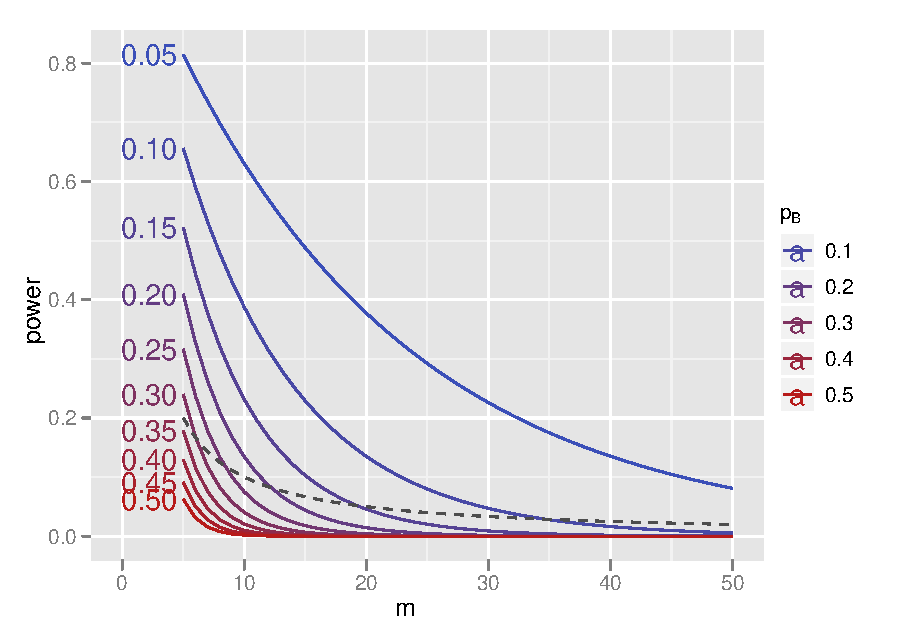
\includegraphics[width=3.5in]{images/p_val_power_m.pdf} 
   \caption{Comparison of probabilities to pick the data plot for different size lineups $m$ and different values for data plot strength $p_D$. The grey line shows probability of picking the data plot under $H_0$. }
   \label{fig:pval_power}
\end{figure}

Now assume that the same lineup plot is evaluated by $K$ independent observers. W.l.o.g. let the last plot be the data plot and plots 1 through $m-1$ the null plots. Let $n_i$ be the number of observers who picked plot $i$ as the plot with the structure least consistent with the null hypothesis, then $\sum_{k=1}^{m} n_k = K$, and $(n_1, n_2, ..., n_m) \sim$ Mult$_{\pi_1, ..., \pi_m}$ with $\sum_i \pi_i = 1$. We can estimate $\pi_i$ as $\widehat{\pi_i} = n_i/K$. 

For the distribution of $n_m$, %the number of times out of $K$ that observers picked the last plot to show the structure least consistent with the null hypothesis, 
we get
\[
n_m\sim \left \{ 
\begin{array}{ll}
B_{K, (1-E[p_D])^{m-1}} & \text { under } H_1\\
B_{K, 1/m} & \text { under } H_0
\end{array}
\right .
\]

Under $H_1$ we therefore get an estimate for the strength of the signal in the test statistic based on a lineup evaluation as 
\begin{equation}\label{eqn:power_estimate}
\widehat{E[p_D]} = 1- \left(\frac{n_m}{K}\right)^{1/(m-1)}.
\end{equation}

\blue{Note that the right hand side of equation (\ref{eqn:power_estimate}) is independent of the parameter $\theta$, but just based on the lineup evaluation by independent observers. This allows us to compute this value independently of the parametric setting. We therefore define the {\it signal strength} of a  visual test as the following:

\begin{dfn} \label{dfn:signal}
The {\it signal strength} $\sigma_T$ of a visual test is defined as the probability to identify the data plot.
\end{dfn}

In a lineup of size $m$, evaluated by $K$ independent observers,  we can estimate the signal strength of the test as
\[
\sigma_T^{m-1} = \frac{n_m}{K}.
\]

In a parametric setting, signal strength of a test coincides with the power of the test.
}

\red{We need to comment on how this ties in to the rest of the paper: this is a theoretical consideration based on the assumption that observers are able to spot the plot with the smallest/a small $p$-value.}

Theoretical power for the regression parameters is derived in the next section.
\section{Inference for a Regression Model} \label{sec:regression}

Consider a linear regression model 
\begin{equation}\label{multi} Y_i = \beta_0 + \beta_1 X_{i1} + \beta_1 X_{i2} + \beta_3 X_{i1}X_{i2} + ... + \epsilon_i 
\end{equation}
where $\epsilon_i \stackrel{iid}{ \sim } N(0,\sigma^2)$, $i=1,2, .., n$. The covariates ($X_j, j=1,..,p$) can be continuous or discrete. 

Suppose $X_k$ is a categorical variable with two levels, and we test the hypothesis $H_0:\beta_k=0$ vs $H_1: \beta_k \ne 0$. If the responses for the two levels of the categorical variable $X_k$ in the model are significantly different and we fit the null model to the observed data, the resulting residual plot shows two groups of residuals. To test this we generate side-by-side boxplots of the residuals conditioned on the two levels of $X_k$, as the test statistic. If $\beta_k\ne 0$ the boxplots show a vertical displacement. 

In a regression setting, there is a multitude of established graphics that help with the evaluation and diagnostics of a model \citep{cook:99}. Table \ref{tbl:stat_multiple} shows an overview of some commonly used charts and their corresponding hypothesis tests. Note that some charts can be associated with several different testing situations. In our paper, we pick the examples for situation 2 and 3 as candidates.

A lineup including the test statistic  for a binary $X_k$ is shown in Figure \ref{fig:test_category}. The 19 null plots are generated  by simulating residuals from $N(0,\hat{\sigma}^2)$. The test statistic, the plot containing the observed data, is randomly placed among these null plots. If the test statistic is identifiable the null hypothesis is rejected. % with a $p$-value of at most 0.05.

\begin{figure}[hbt]
%\begin{figurehere}
   \centering
       \scalebox{0.95}{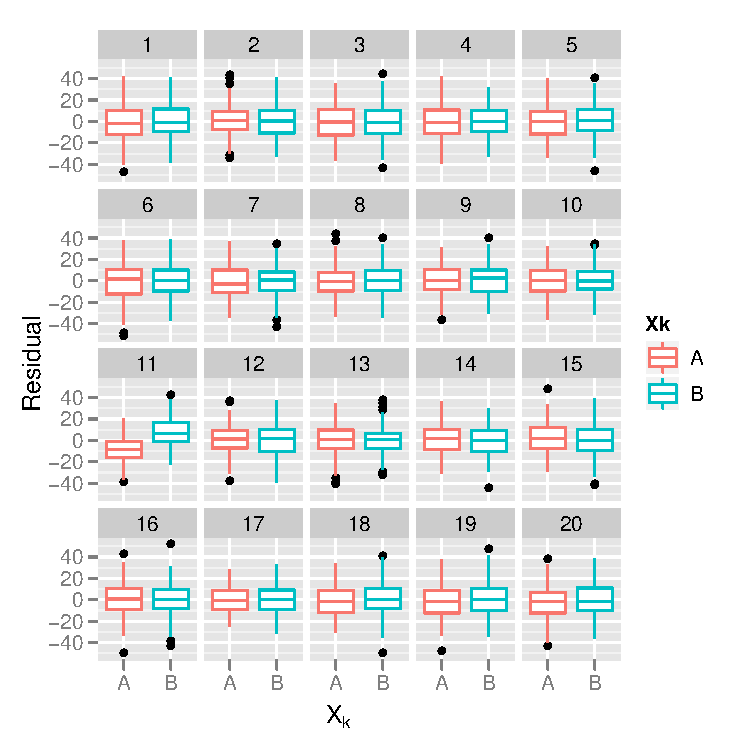
\includegraphics{test_category.pdf}}
       \caption{Lineup plot ($m=20$) for testing $H_0: \beta_k=0$. When the alternative hypothesis is true the plot of the observed data should show a vertical displacement between box plots. Which plot has the biggest vertical displacement between the boxplots?}
       \label{fig:test_category}
\end{figure}
%\end{figurehere}

\begin{table*}[hbtp] 
\caption{Test Statistics for Testing Hypothesis Related to Model $Y_i = \beta_0 + \beta_1 X_{i1} + \beta_1 X_{i2} + \beta_3 X_{i1}X_{i2} + ... + \epsilon_i  $ } 
\centering 
\begin{tabular}{m{0.5cm}m{3cm}m{2.5cm}m{2.6cm}m{5.5cm}} 
\hline\hline 
Case & Null Hypothesis & Statistic & Test Statistic & Description \\ [0.5ex] % inserts table %heading 
\hline 
1 & $H_0: \beta_0=0$ & Scatter plot & \begin{minipage}[t]{2cm}\begin{center}  	\scalebox{0.1}{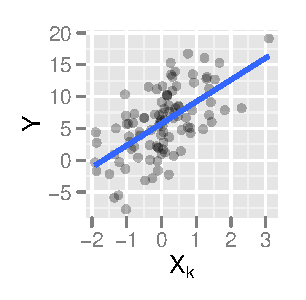
\includegraphics{stat_intercept.pdf}} \end{center} \end{minipage} & Scatter plot with least square line overlaid. For lineup plot, we simulate data from fitted null model. \\ 
2 & $H_0: \beta_k=0$ & Residual plot & \begin{minipage}[t]{2cm}\begin{center}  	\scalebox{0.1}{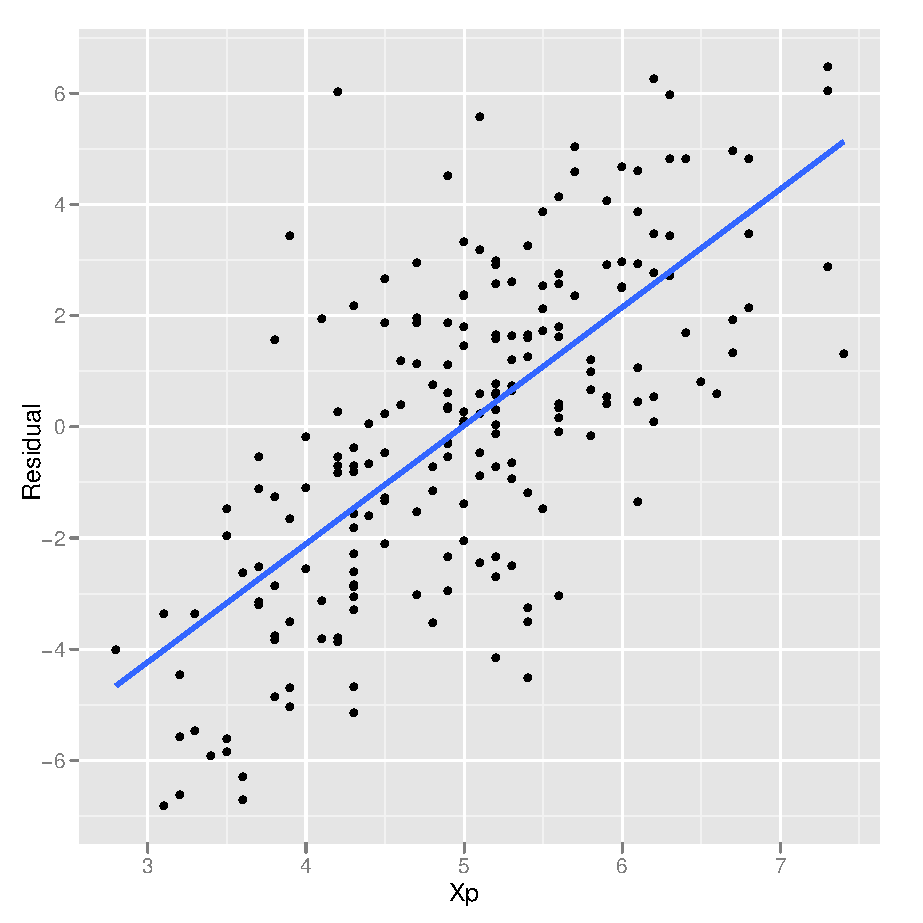
\includegraphics{stat_bet_p.pdf}} \end{center} \end{minipage} & Residual vs $X_k$ plots. For lineup plot, we simulate data from normal with mean 0 variance $\hat{\sigma}^2$. \\ 
3 & $H_0: \beta_k=0$ (for categorical $X_k$) & Box plots of residuals & \begin{minipage}[t]{2cm}\begin{center}  	\scalebox{0.18}{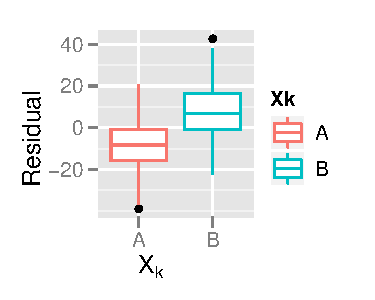
\includegraphics{stat_category.pdf}} \end{center} \end{minipage} & Box plot of residuals grouped by category of $X_k$. For lineup plot, we simulate data from normal with mean 0 variance $\hat{\sigma}^2$. \\
4 & $H_0: \beta_k=0$ (interaction with categorical $X_k$) & Scatter plot & \begin{minipage}[t]{2cm}\begin{center}  \scalebox{0.11}{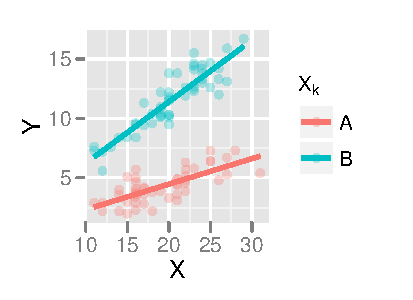
\includegraphics{stat_interection.pdf}} \end{center} \end{minipage} & Scatter plot with least square lines of each category overlaid. For lineup plot, we simulate data from fitted null model.\\[1ex] % [1ex] adds vertical space 
5 & $H_0: X$ Linear & Residual Plot & \begin{minipage}[t]{2cm}\begin{center}  	\scalebox{0.1}{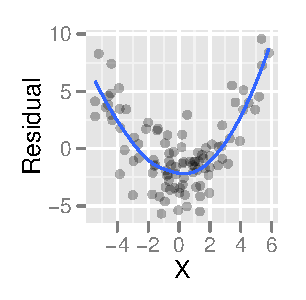
\includegraphics{stat_nonlinear.pdf}} \end{center} \end{minipage} & Residual vs predictor plots with loess smoother overlaid. For lineup plot, we simulate residual data from normal with mean 0 variance $\hat{\sigma}^2$. \\ 
6 & $H_0: \sigma^2=\sigma^2_0$ & Box plot & \begin{minipage}[t]{2cm}\begin{center}  \scalebox{0.15}{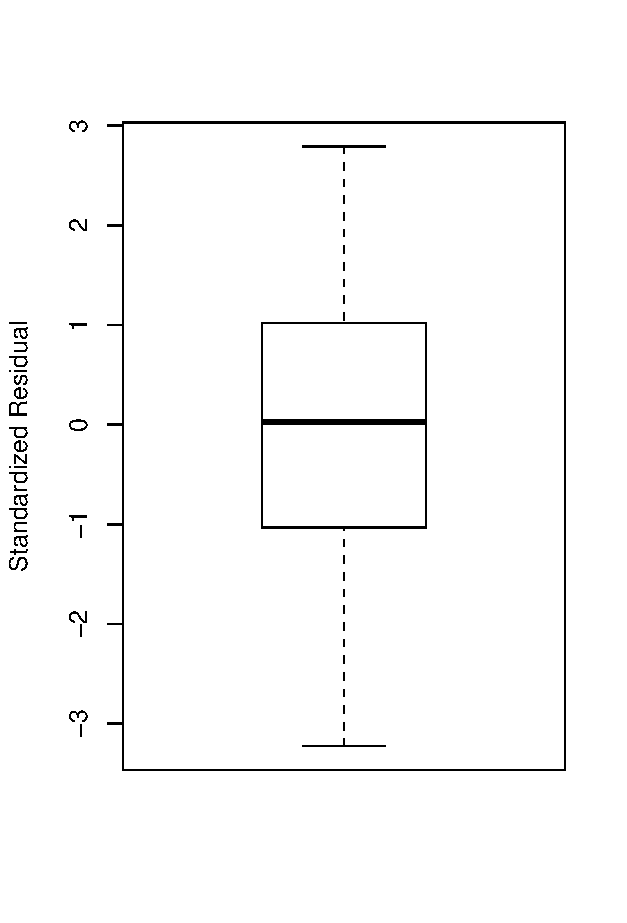
\includegraphics{stat_sigma_box.pdf}} \end{center} \end{minipage} & Box plot of standardized residual divided by  $\sigma^2_0$. For lineup plot, we simulate data from standard normal. \\ 				
7 & $H_0: \rho_{X,Y|Z}=\rho$ & Scatter Plot & \begin{minipage}[t]{2cm}\begin{center}  	\scalebox{0.1}{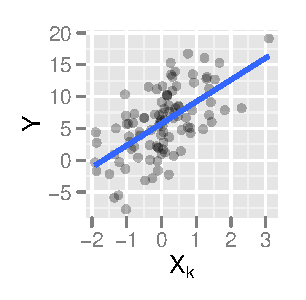
\includegraphics{stat_intercept.pdf}} \end{center} \end{minipage} & Scatter plot of Residuals obtained by fitting partial regression. For lineup plot, we simulate data (mean 0 and variance 1) with specific correlation $\rho$. \\ 
8 & $H_0:$ Model Fits & Histogram & \begin{minipage}[t]{2cm}\begin{center}  \scalebox{0.1}{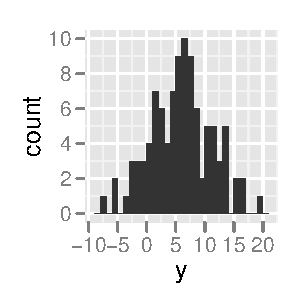
\includegraphics{stat_goodness_simple.pdf}} \end{center} \end{minipage} & Histogram of the response data. For lineup plot, we simulate data from fitted model. \\[1ex] % [1ex] adds vertical space 
9 & Special case $p=1$ $H_0: \rho_{X,Y} =\rho$ & Scatter plot & \begin{minipage}[t]{2cm}\begin{center}  \scalebox{0.1}{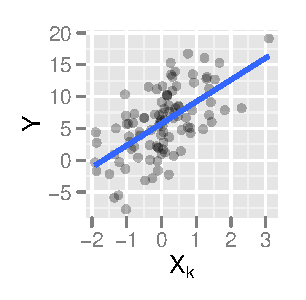
\includegraphics{stat_intercept.pdf}} \end{center} \end{minipage} & Scatter plot with least square line overlaid For lineup plot, we simulate data with correlation $\rho$.\\			
\hline 
\end{tabular} 
\label{tbl:stat_multiple} 
\end{table*} 




%\subsection{Expected power}

% Di: This is specific for the regression model
%Consider the hypothesis test $H_0: \beta_k=0$ against $H_1: \beta_k \ne 0$ in model \ref{multi}.
%%Now consider estimating the power of the visual test. 
%%Suppose $F_{|t|}(.)$ is the distribution function of an absolute value of $t$. For the regression slope parameter $\beta$ suppose the associated test statistic in classical test be $t_{obs}$ with $p$-value $p_B$. By definition we have 
%%
%%$$p_B=Pr(|t| \ge t_{obs}| H_0)=1-F_{|t|}(t_{obs}) \Rightarrow |t_{obs}|=F_{|t|}^{-1}(1-p_B)$$
%%
%%\red{HH: the following paragraph should probably move up, but I'm not sure how to change it appropriately. Mahbub, could you take care of that?}
%%Now suppose $F_{|t|}(.;\delta)$ denotes the distribution function of an absolute value of $t$ distribution with non-centrality parameter $\delta$. Thus the distribution function of $p-value$ be  
%%\begin{eqnarray}\label{dist_p}
%%F{p_B}(p) &=& Pr(p_B \le p)=1-Pr(1-p_B \le 1-p) \nonumber \\
%%  &=& 1-Pr(F_{|t|}^{-1}(1-p_B) \le F_{|t|}^{-1}(1-p) ) \nonumber \\
%%  &=& 1-Pr(|t_{obs}| \le F_{|t|}^{-1}(1-p)) \nonumber \\
%%  &=&\left\{ \begin{array}{ll}
%%          1-F_{|t|}( F_{|t|}^{-1}(1-p))=p &\mbox{ ; under $H_0$} \\
%%          1-F_{|t|}( F_{|t|}^{-1}(1-p); \delta) &\mbox{ ; under $H_1$} 
%%       \end{array} \right.     
%%\end{eqnarray}
%%
%%Thus the density of $p_B$ is Uniform(0,1)  under $H_0$. As noted by \cite{Ruppert:2007}, under $H_1$ the density $$f_{P_B}(p_B; \delta)= \frac{f_{|t|}(F_{|t|}^{-1}(1-p_B);\delta)}{f_{|t|}(F_{|t|}^{-1}(1-p_B))}$$ derived from equation \ref{dist_p}  is a right skewed distribution.  
%In a lineup plot we simulate $m-1$ residual data sets from null model where each of these $m-1$ null data sets produces a corresponding $p$-value $p_{0,i}$ and $p_{0,i} \sim \text{Uniform}(0,1)$ for $i = 1, ..., m-1$. Suppose  $p_0=\min_i(p_{0,i})$. Thus $p_0 \sim \text{Beta}(1,m-1)$. 

Under the assumption that an observer is able to pick the plot with the smallest $p$-value from a lineup plot,  this leads to the decision to reject $H_0$ when $p_{B} < p_0$. Thus we have the expected power as 

\begin{equation}\label{power_exp} 
   Power(\beta)=Pr(p_{B} < p_0)  \quad \text{for}  \quad \beta \ne 0
\end{equation}

Figure \ref{fig:power_expected} shows the power of the uniformly most powerful test (UMP) in comparison to the expected power of the visual test obtained from equation \eqref{power_exp}. Notice that the expected power of the visual test is almost as good as the power of UMP test. In fact, the only loss we experience stems from comparing the test statistic to only a discrete number of  $m-1$ samples from the null distribution. 

%Theorem \ref{thm:power} helps to compute the expected power of visual inference.
%\begin{thm}\label{thm:power}
% Equation \ref{power_exp}  yields expected power of visual inference as Power($\beta$) = $E(1-p_B)^{m-1}$ .
%\end{thm}
% 
%{ \em proof}
%
%Since $p_0 \sim \text{Beta}(1,m-1)$,  for $t \in (0,1)$ we have the distribution function of $p_0$ be
%\begin{eqnarray*}
%F{p_0}(t) &=& (m-1) \int_0^t{(1-p_0)^{(m-2)}dp_0} \\
%  &=&  -(m-1) \int_1^{1-t}{x^{(m-2)}dx}\\
%  &=& \left[ x^{m-1}\right]^1_{1-t}\\
%  &=&1-(1-t)^{m-1} \rightarrow 1 \quad \text{as} \quad m \rightarrow \infty
%\end{eqnarray*}
%
%% verified this computation from http://www.wolframalpha.com using command int (m-1)*(1-p)^(m-2) dp, p=0,t
%
%Thus expected power in equation \ref{power_exp} be
%\begin{eqnarray*}
% Pr(p_{B} < p_0) &=& 1- Pr( p_0 \le p_{B} ) \\
%  &=& 1- \int_{0}^{1}{Pr( p_0 \le p_{B} |p_{B} =t) f_{p_{B} }(t)dt } \\
%  &=& 1-  \int_{0}^{1}{F{p_0}(t) f_{p_{B} }(t)dt } \\
%  &=& E(1-p_B)^{m-1}   \\
%%  & \rightarrow &1-  \int_{0}^{1}{ f_{p_{B} }(t)dt }  = F_{p_B}(0) \quad \text{as} \quad m \rightarrow \infty
%\end{eqnarray*}
%
%
\begin{figure}[hbtp]
   \centering
       \scalebox{.65}{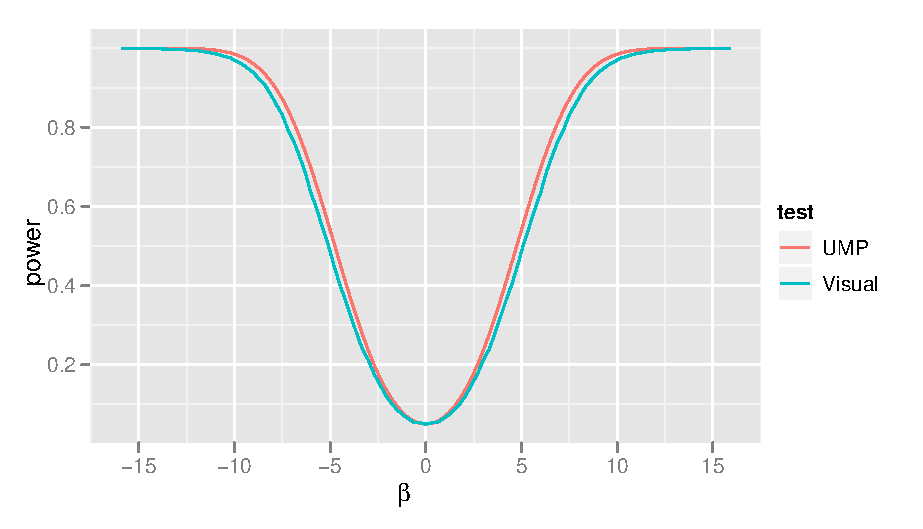
\includegraphics{power_expected.pdf}}
       \caption{Expected power of visual test  and the power of UMP test for sample size $n =100$ and $\sigma = 12$.}
       \label{fig:power_expected}
\end{figure}

% \pagebreak

% -------- Heike's writeup added here

%\subsection{Some Power Considerations}


%\subsection{Expected number of choices}
%Since $X$ has a binomial distribution, we can have a look at the number of plots among the null plots that we would expect to be picked over the data plot:
%\[
%E[X] = (m-1)(1-E[p_B]).
%\]
%With an increase of the lineup size $m$ the number of null plots with a potentially stronger signal than the data plot grows linearly.
%This should allow us to infer some of the signal strength $p_B$ as
%\begin{equation} \label{plot_signal}
%E[p_B] = 1 - E[X]/(m-1),
%\end{equation}
%i.e. by averaging over the number of plots with  a stronger signal than the data plot we can evaluate signal strength of the plot even in the case where the data plot is not being picked by the observer.
%


\subsection{Estimating Power from Lineups}

We estimate the empirical power from responses on a specific lineup plot  generated with known values of sample size ($n$), variance ($\sigma^2$) and regression parameter ($\beta$) in model \ref{multi}. Suppose, we have responses from $N$ independent observers with $u$ identifications of the observed plot. This gives an estimated power of
\begin{equation}\label{power_est} Power(\beta)=\frac{u}{N} \hspace{1cm} 0 \le u \le N \end{equation}

Suppose each of $N$ independent observers gives evaluations on multiple lineup plots and responses are associated with binary random variable $Y_{ij}$. Let $Y_{ij} = 1$, if subject $j$ correctly identifies the test statistic on lineup $i$, and 0 otherwise.
We model $\pi_{ij} = E(Y_{ij})$ as  a mixed effects logistic regression

\begin{equation}
g(\pi_{ij}) = X_{ij}B  + Z_{ij} \tau_j 
\label{mixed} 
\end{equation}
%
where $\tau_j$ is random effects coefficient vector of length $q$ for subject $j$,  $\tau_j  \sim  MVN(0,\Sigma)$ with variance covariance matrix $\Sigma$, $Z_{ij}$ is the $i$th row vector of random effects covariates for subject $j$, $B$ is a vector of coefficient of length $p$, the number of fixed effect covariates being used, $X_{ij}$ is the $i$th row vector of the fixed effects covariates for subject $j$ and logit link function $g(\pi)=\log(\pi) - \log(1-\pi); 0 \le \pi \le 1$. The covariates could be demographic information of people such as age, gender, education level etc. as well as sample size ($n$), regression parameter ($\beta$) and variance ($\sigma^2$) of model \ref{multi}. 

From model \ref{mixed} we obtain %$\pi=Pr(Y=1|X_1, X_2, ..., X_p)$, 
the power of the underlying testing procedure as a population average %by ignoring the random effect part. 
%Thus we have the overall probability of success ($\pi$ or power) 
for specified sample size ($n$) and  variance ($\sigma$)  as 

\begin{equation}\label{eqn:power} 
Power(\beta) = \pi=Pr(Y=1|\beta, n, \sigma) 
\end{equation}


\section{Simulation Experiment} \label{sec:simulation}

\subsection{Experiment with a discrete covariate}

The experiment is designed to study the ability of human observers to detect the effect of a single variable $X_2$ (corresponding to parameter $\beta_2$) in a two variable ($p=2$) regression model (Equation \eqref{multi}). Data is simulated for different values of $\beta_2 (=0, 1, 3, 5, 7, 8, 10, 16)$, with two sample sizes ($n=100, 300$) and two standard deviations of the error ($\sigma=5, 12$). The set of $\beta_2$ values was chosen so that estimates of the power should produce reasonable power curves, comparable to the theoretical UMP test. We fixed the values of $\beta_0 = 5$,  $\beta_1=15$ and values for $X_1$ were generated as a random sample from a Poisson(30) distribution. Data sets with different combinations of $\beta_2$,  $n$ and $\sigma$ were generated with frequencies shown in Table \ref{tbl:experiment_params}. Three replicates of each level were generated. These produced 60 different ``observed data sets''. 




\begin{table}[hbtp]
\caption{Values of parameters considered for three survey experiments} % title name of the table
\centering
% centering table
\begin{tabular}{c c l l l}
% creating 10 columns
\hline\hline

% inserting double-line
& & \multicolumn{3}{c}{values for slope ($\beta$)} \\
 \cline{3-5}

\raisebox{1.5ex}  {Sample size ($n$)} &   \raisebox{1.5ex} {$\sigma$} &  \multicolumn{1}{c} {Experiment 1}  & \multicolumn{1}{c} {Experiment 2}  & \multicolumn{1}{c} {Experiment 3}
\\ [0.5ex]
\hline
% inserts single-line

% Entering 1st row
&  5 & 0, 1,  3, 5, 8  & 0.25, 0.75, 1.25, 1.75, 2.75 & 0.1, 0.4, 0.75, 1.25, 1.5, 2.25\\[-1ex]
\raisebox{1.5ex}{100} &12
& 1, 3, 8, 10, 16  & 0.5, 1.5, 3.5, 4.5, 6 &\\[1ex]

% Entering 2rd row
&  5 & 0, 1, 2, 3, 5  & 0.1, 0.4, 0.7, 1, 1.5&\\[-1ex]
\raisebox{1.5ex}{300} & 12
& 1, 3, 5, 7, 10  & 0, 0.8, 1.75, 2.3, 3.5 &\\[1ex]
% [1ex] adds vertical space
\hline
% inserts single-line
\end{tabular}
\label{tbl:experiment_params}
\end{table} 


For added control, to ensure a signal in the simulated observed data a blocking structure was used to filter data sets. A 1000 sets were generated for each parameter combination and the traditional $t$-statistic and $p$-value associated with $H_0: \beta_2=0$ were calculated. The 3 replicates were drawn from each of three blocks of $p$-values: (0.0-$q_{33}$), ($q_{33}$-$q_{66}$), ($q_{66}$-1) where $q_i$ is the $i$th percentile in the distribution of the $p$-values. Additional control was applied to the 19 null plots. Because the distribution of these $p$-values should follow a Uniform(0,1) distribution, data sets were binned on this range by $p$-value, and a data set was randomly selected from each bin.
  

\subsection{Experiment with a continuous covariate} 

This experiment is designed for the same regression model (Equation \eqref{multi}) with $p=1$ and covariate $X_1$ being continuous. Data is simulated with two sample sizes ($n=100, 300$) and two standard deviations of the error ($\sigma=5, 12$). The different values for slope parameter that are used to generate data are shown in Table \ref{tbl:experiment_params}. We arbitrarily fix $\beta_0 = 6$ while generating observed data. For each combination of parameter, we generate at least three different observed data sets constituting a total of 65 lineups. 


\subsection{Experiment with contaminated data}

The first two simulation experiments are based on normal error model which satisfies the conditions for uniformly most powerful (UMP) test. To study how the proposed visual inference work for a scenario where the data are not really coming from a normal model we design a contaminated data experiment. To generate the contaminated data set of size $n=100$ we used the following model


\[
  Y_i = \left\{
  \begin{array}{l l}
    5+\beta X_i + \epsilon_i  & \quad  X_i \sim N(0,1) \quad \text{ $i$ =1,...,85}\\
    15+ \eta_i & \quad X_i \sim N(\mu,1/3) \quad  i=86,...,n\\
  \end{array} \right.
\]
where $\epsilon_i \stackrel{iid}\sim N(0,\sigma)$, $\eta_i \stackrel{iid}\sim N(0,\sigma/3)$ and $\mu = -1.75$. One such plot of the contaminated data for $\sigma$=5 and $\beta$=5 is shown in figure \ref{fig:cont_dat}. For this experiment we only consider sample size $n=100$ and error standard deviation $\sigma=5$.

For this experiment we generate five replications of observed data sets for each slope value shown in table \ref{tbl:experiment_params}. This produces 30 lineups.

\begin{figure}[hbt]
%\begin{figurehere}
   \centering
       \scalebox{0.4}{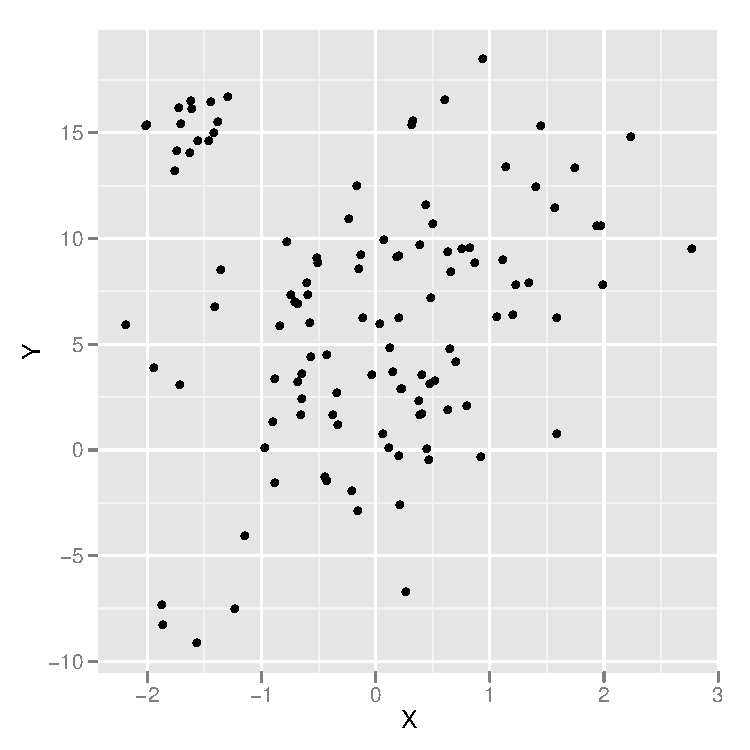
\includegraphics{contaminated_data.pdf}}
       \caption{Scatterplot of a simulated contaminated data set generated such that a simple linear model produce a slope almost negligible, ie, if we fit model (Equation \eqref{multi}) with $p=1$  to this data, the resulting estimate of $\beta_1$ would not be statistically significant.
}
       \label{fig:cont_dat}
\end{figure}


\begin{figure*}[hbtp]
   \centering
       \scalebox{0.6}{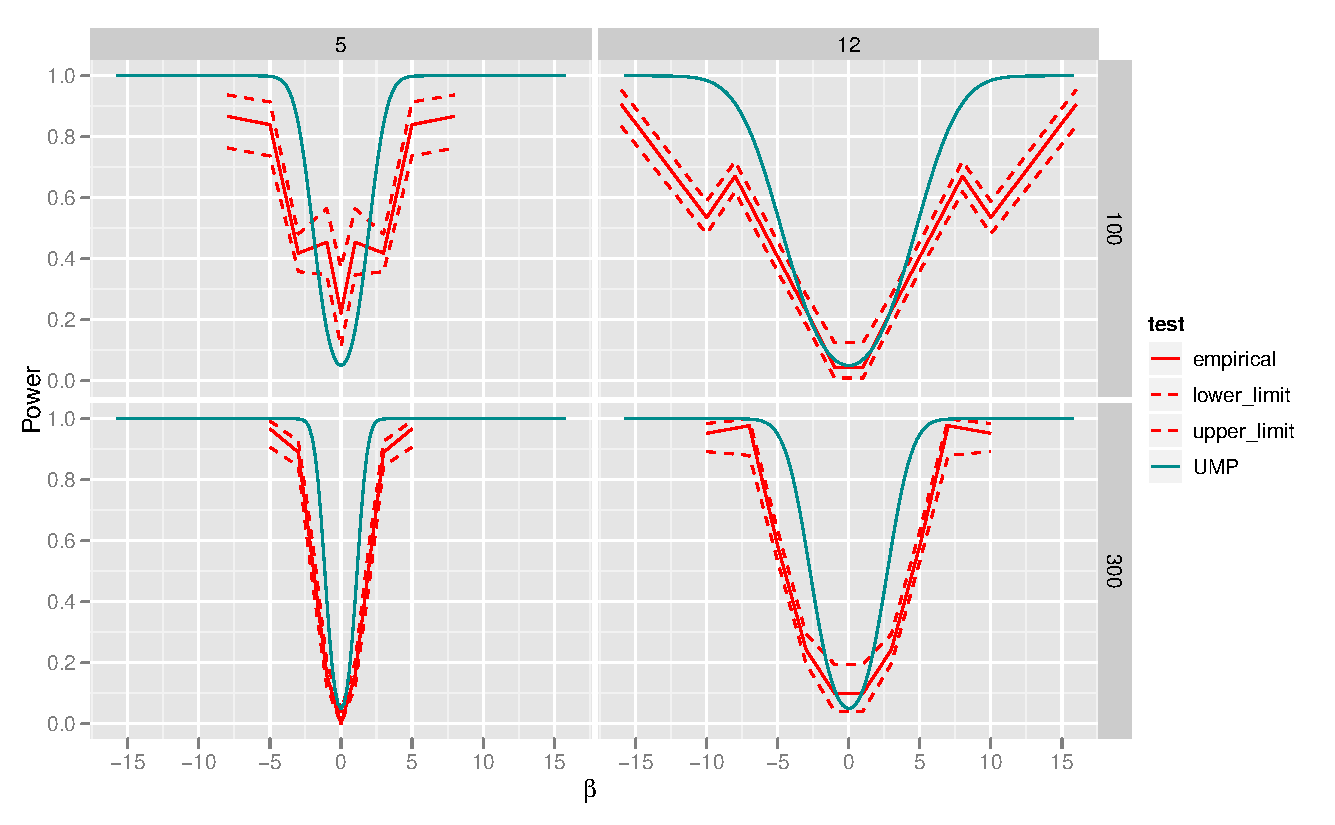
\includegraphics{power_observed.pdf}}
       \caption{Observed power of visual test from equation \eqref{power_est} with pointwise 95\% confidence limits and the power of UMP test for sample size $n= 100,300$ and $\sigma = 12,5$ as per experiment 1.}
       \label{fig:power_observed}
\end{figure*}


\begin{figure*}[hbtp]
   \centering
       \scalebox{0.7}{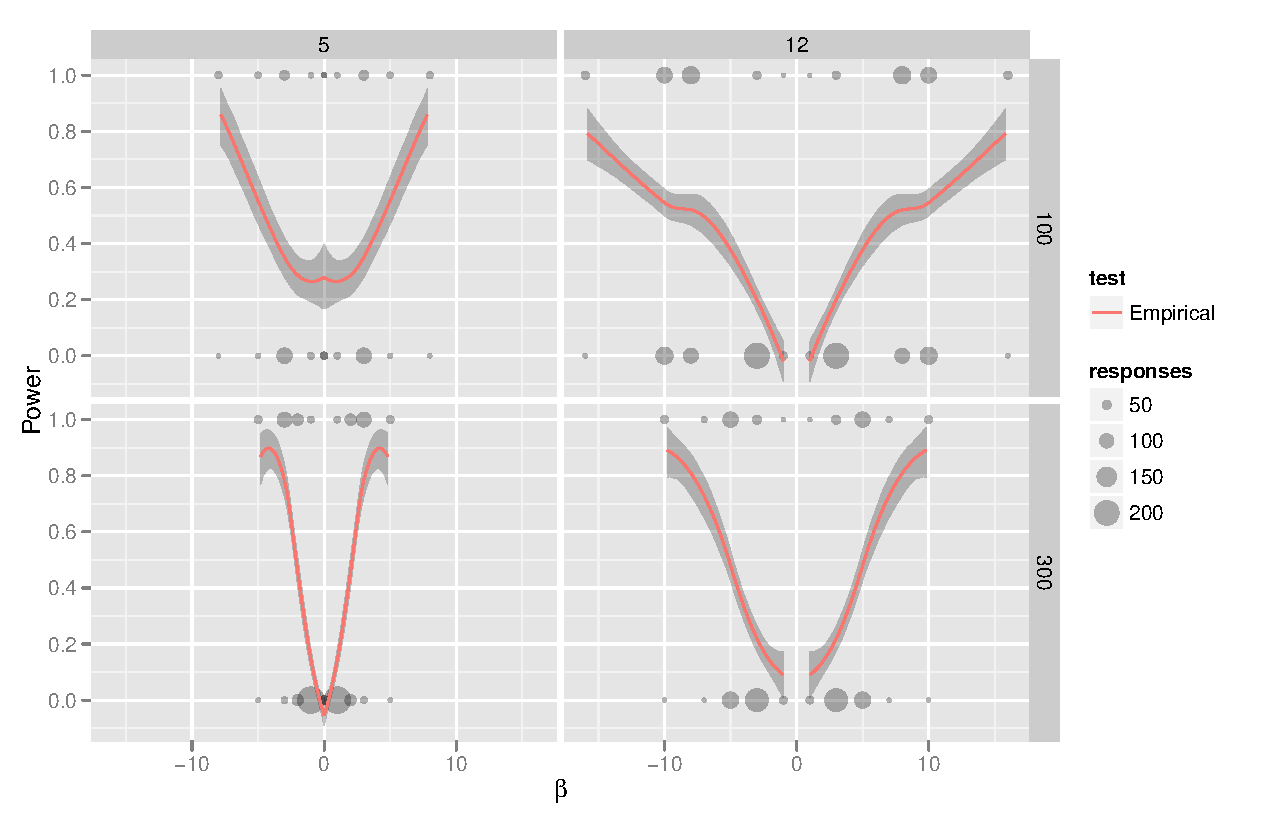
\includegraphics{power_loess_exp1.pdf}}
       \caption{Observed power shown by loess smoother with simultaneous bootstrap confidence band and the power of UMP test for sample size $n= 100,300$ and $\sigma = 12,5$ as per experiment 1.}
       \label{fig:power_loess1}
\end{figure*}


\begin{figure*}[hbtp]
   \centering
       \scalebox{0.7}{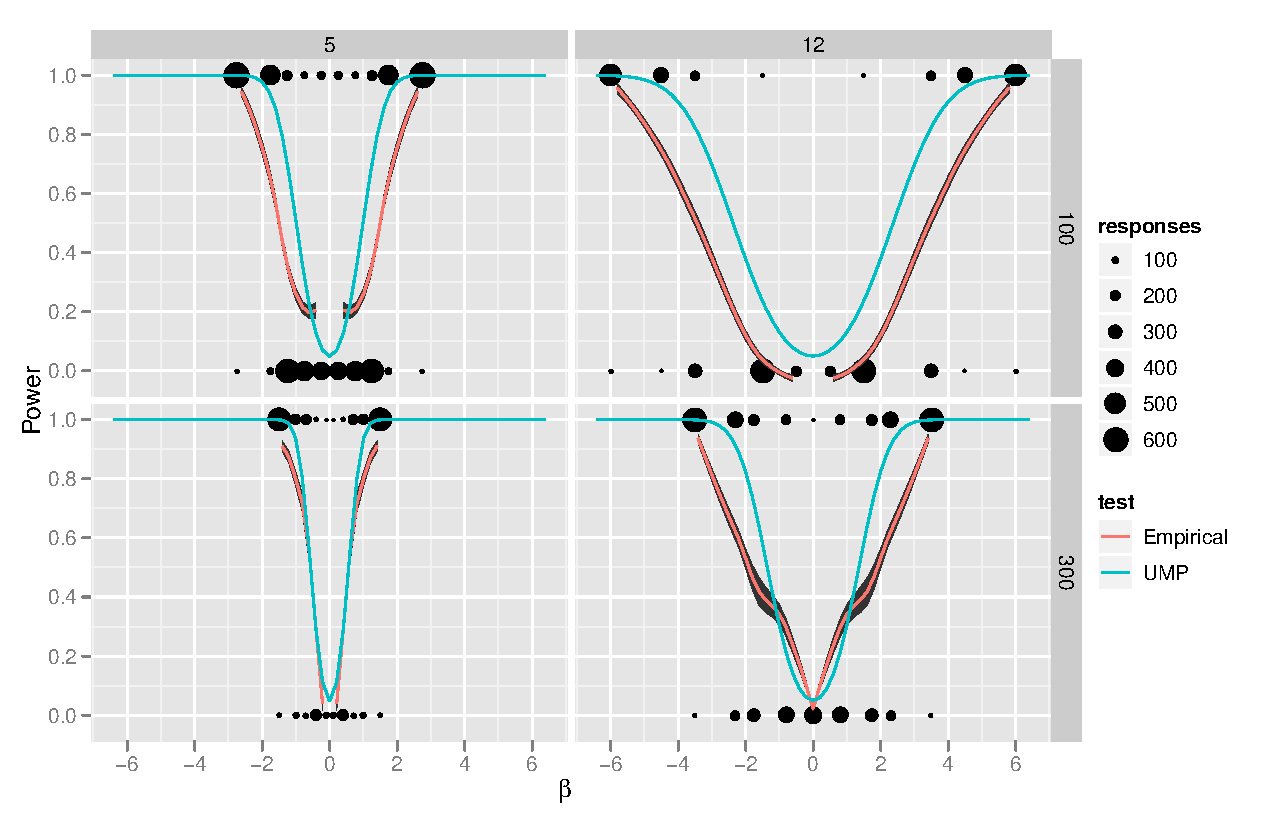
\includegraphics{power_loess_exp2.pdf}}
       \caption{Observed power shown by loess smoother with simultaneous bootstrap confidence band and the power of UMP test for sample size $n= 100,300$ and $\sigma = 12,5$ as per experiment 2.}
       \label{fig:power_loess2}
\end{figure*}


\begin{figure*}[hbtp]
   \centering
       \scalebox{0.4}{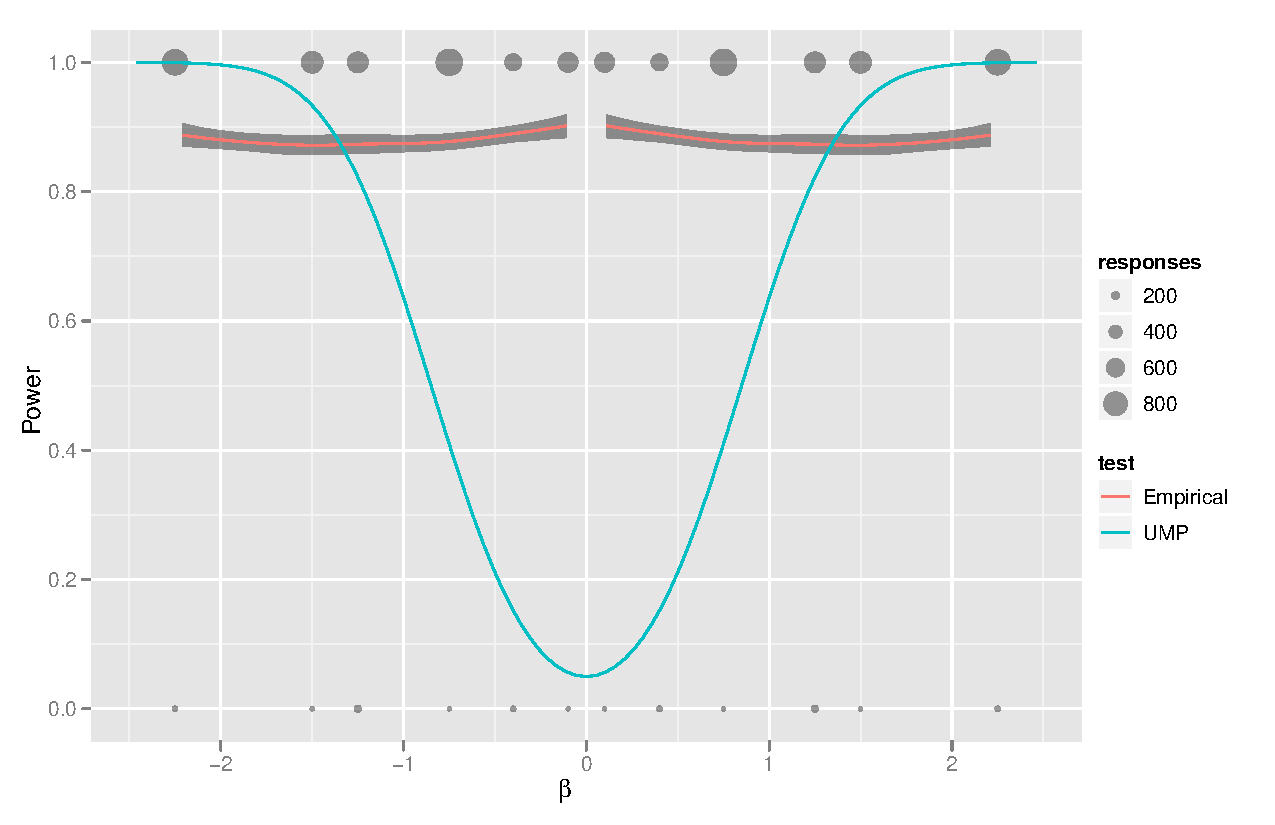
\includegraphics{power_loess_exp3.pdf}}
       \caption{Observed power shown by loess smoother with simultaneous bootstrap confidence band and the power of UMP test for sample size $n= 100$ and $\sigma = 5$ as per experiment 3. Notice that for experiment 3, power does not seem to depend on the parameter $\beta$. Di/Heike, I am not sure how I can relate this to demonstrate the power of visual inference when normal conditions are not met. Does this really test our hypothesis $H_0: \beta=0$ or some other hypothesis about the existence of cluster in the data?}
       \label{fig:power_loess3}
\end{figure*}


\begin{figure*}[hbtp]
   \centering
       \scalebox{0.7}{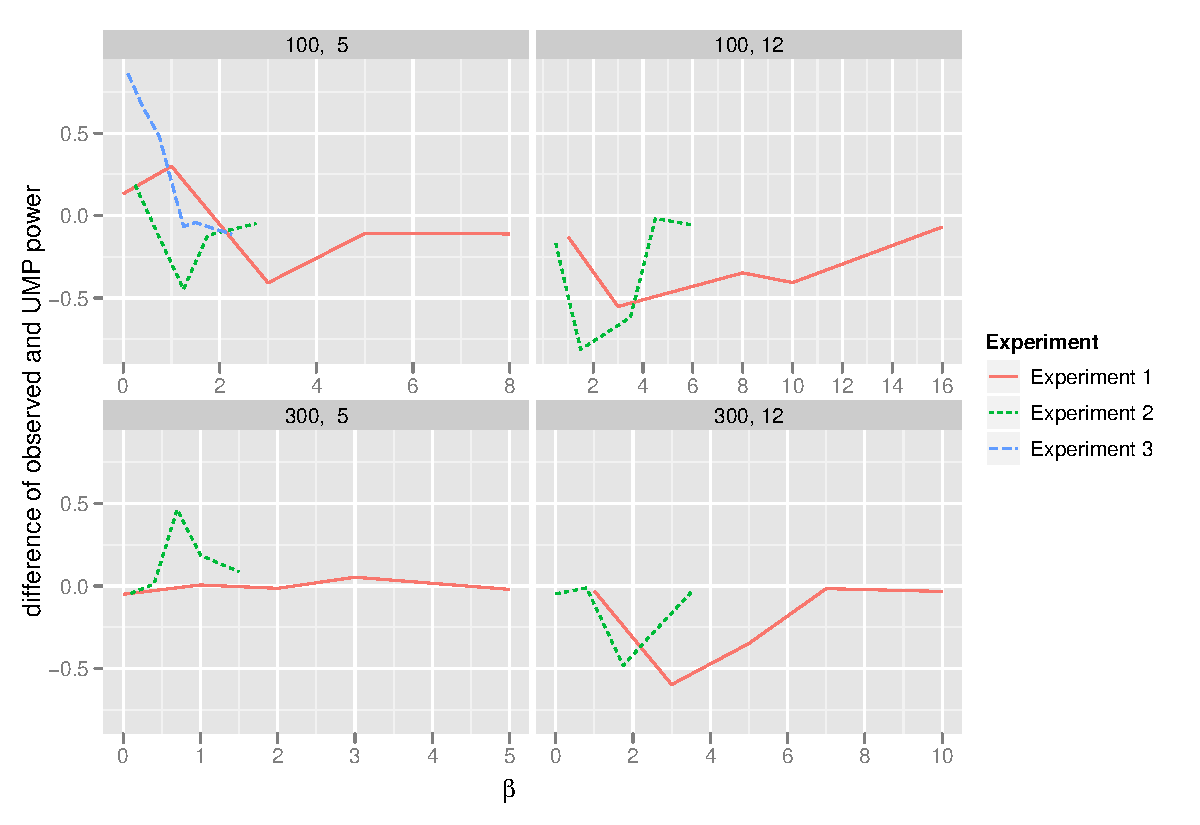
\includegraphics{power_diff_exp.pdf}}
       \caption{Difference of Observed power from UMP test power obtained in three experiments for sample size $n= 100,300$ and $\sigma = 12,5$ and values of slope parameter $\beta$ as shown in table \ref{tbl:experiment_params}.}
       \label{fig:power_diff_exp}
\end{figure*}


\begin{figure*}[hbtp]
   \centering
       \scalebox{0.6}{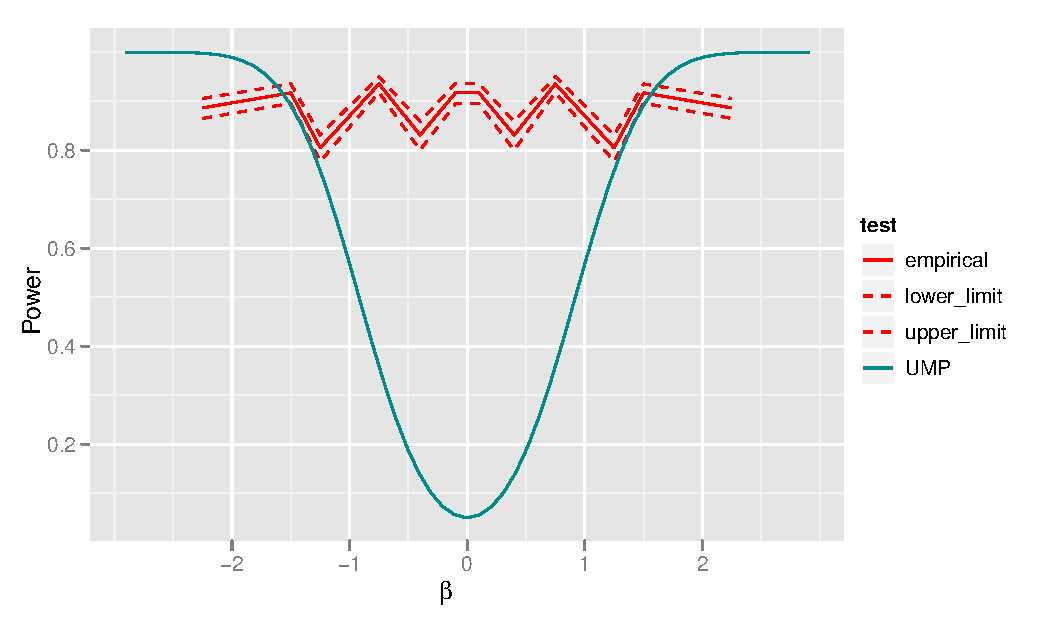
\includegraphics{power_observed_exp3.pdf}}
       \caption{Observed power of visual test from equation \eqref{power_est} with pointwise 95\% confidence limits and the power of UMP test for sample size $n= 100$ and $\sigma = 5$ as per experiment 3. }
       \label{fig:power_observed_exp3}
\end{figure*}


\begin{figure*}[hbtp]
   \centering
       \scalebox{0.6}{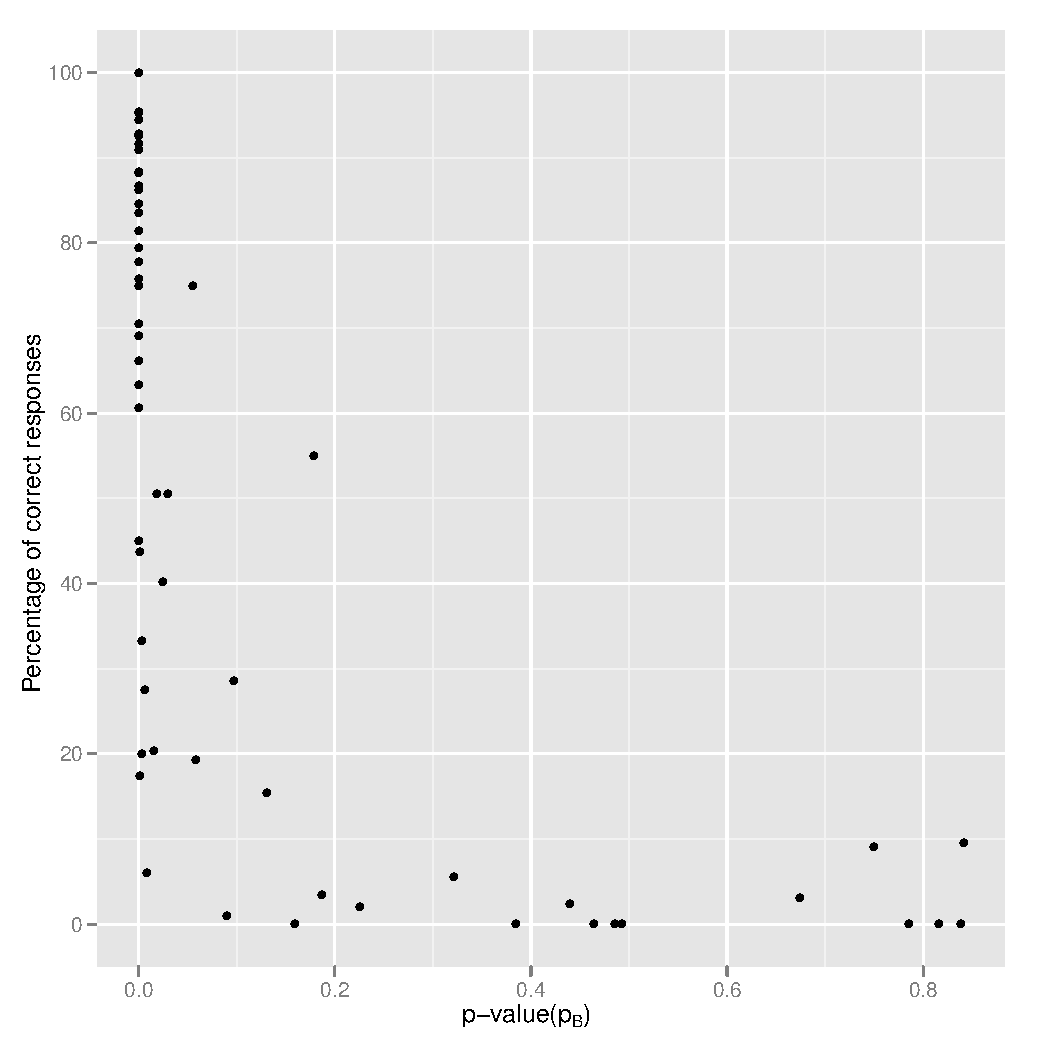
\includegraphics{p_val_percent_correct.pdf}}
       \caption{Percentage of correct responses decreases rapidly with the increase of p-value. After p-value exceeds 1.5 it is very unlikely to identify the observed plot. The theoretical justification of this is shown in figure \ref{fig:pval_power}}
       \label{fig:pval_pcorrect}
\end{figure*}

\begin{figure*}[hbtp]
   \centering
       \scalebox{0.6}{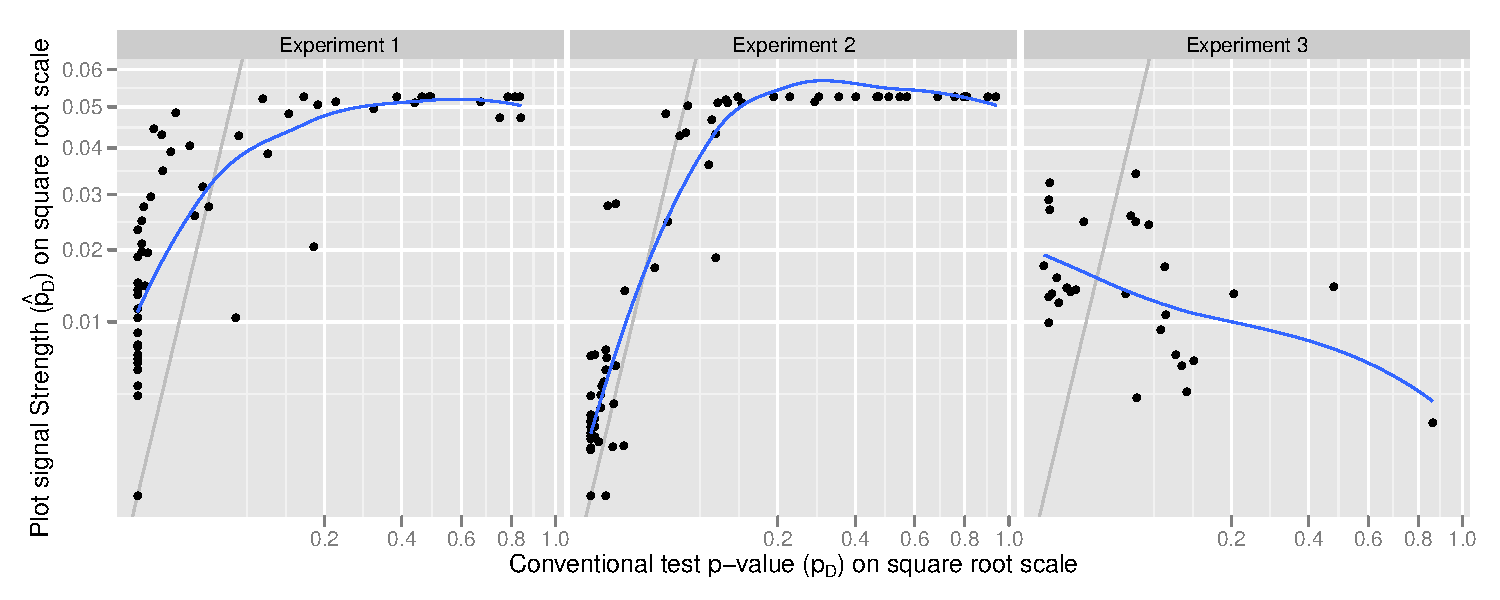
\includegraphics{p_val_plot_signal.pdf}}
       \caption{p-value vs plot signal strength. The solid line represents 45 degree line which represents the equity shown in equation \eqref{plot_signal}}
       \label{fig:pval_plot_signal}
\end{figure*}




Participants for all the experiments were recruited through \cite{turk} Amazon's Mechanical Turk. Each participant was shown a sequence of 10 lineup plots. Participants are asked to select the plot with the biggest vertical difference, give a reason for their choice, and determine a level of  confidence for their decision. Gender, age, education and geographic location of each participant are also collected.
 In total, 3629 lineups were evaluated by 324 people coming from many different locations across the globe.  The results of the experiment are summarized in Figure \ref{fig:power_observed} which shows the observed power from the survey data calculated using equation \eqref{power_est} along with 95\% confidence interval calculated using Fisher's exact method.

\begin{figure}[hbtp]
   \centering
       \scalebox{0.40}{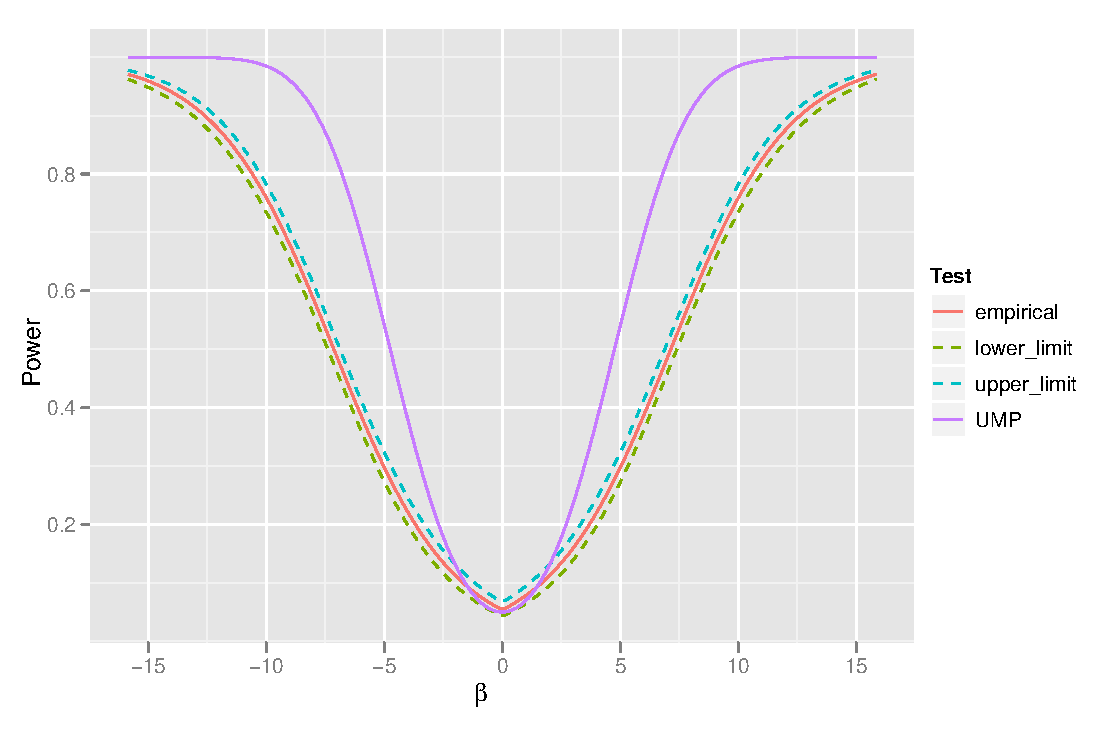
\includegraphics{power_model.pdf}}
       \caption{Estimated power curve from equation \eqref{eqn:power} along with 95\% confidence interval for sample size $n$ = 100 and $\sigma$ = 12.  The corresponding power curve for Uniformly Most powerful (UMP) test is shown for comparison.}
       \label{fig:power_model}
\end{figure}

We fit model \eqref{mixed} to the survey data obtained from the simulation experiment. The estimated overall power curve obtained from equation \eqref{eqn:power} is shown in Figure \ref{fig:power_model}. Model \ref{mixed} also gives the subject specific power curves shown in Figure \ref{fig:power_subject}. The plot includes 20 randomly selected subject-specific power curves. Notice that the power curve estimated for one subject is above the UMP test power curve. 

\begin{figure}[hbtp]
   \centering
       \scalebox{0.45}{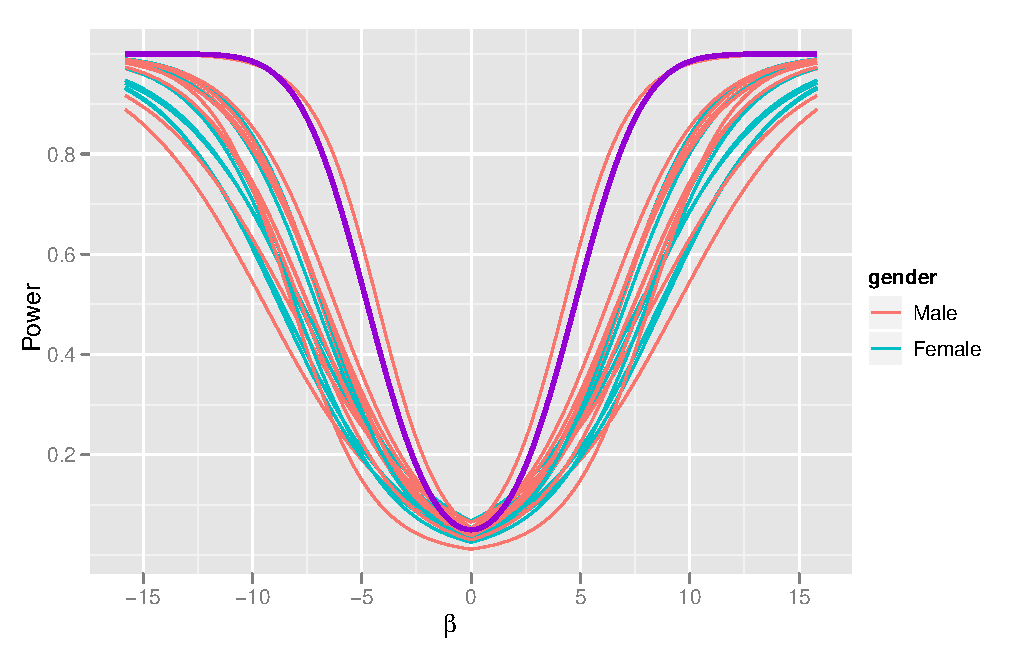
\includegraphics{power_subject.pdf}}
       \caption{Estimated subject specific power curve from model \ref{mixed} for sample size $n$ = 100 and $\sigma$ = 12.  The corresponding power curve for Uniformly Most powerful (UMP) test is shown for comparison.}
       \label{fig:power_subject}
\end{figure}


\section{Conclusions}

The purpose of this paper has been to examine the effectiveness of visual inference methods in direct comparison to existing inference methods. We need to be clear that this is not the purpose of visual inference generally: visual methods should not be seen as competitors to traditional inference.  The purpose here, is to  establish properties and  efficacy of visual testing procedures in order to use them in situations where traditional tests cannot be used. For this experiment the effect of $\beta_2$ was examined using side-by-side boxplots. Future experiments will be conducted to compare other regression parameters as described in Table \ref{tbl:stat_multiple} and assess sensitivity of power to modeling conditions.

\paragraph{Acknowledgement:}

This work was funded by National Science Foundation grant DMS 1007697.

%\bibliographystyle{plain}
%\bibliographystyle{plainnat}
\bibliographystyle{asa}
%\bibliographystyle{ieeetr}
\bibliography{references}

%\end{multicols}


\end{document}  %End of document.





\begin {abstract} 
Statistical graphics play a crucial role in exploratory data analysis, model checking and diagnosis. Until recently there were no formal visual methods in place for determining statistical significance of findings. This changed, when Buja et al.(2009) conceptually introduced two protocols for formal tests of visual findings. In this paper we take this a step further by comparing the lineup protocol (Buja et al.2009) against classical statistical testing  of the significance of regression model parameters. A human subjects experiment is conducted using simulated data to provide controlled conditions. Results suggest that the lineup protocol provides results equivalent to the uniformly most powerful (UMP) test and for some scenarios yields better power than the UMP test.
\end {abstract}

\end{document}
